% Chapter Template

\chapter{A Body of Original Work} % Main chapter title

\label{Chapter3} % Change X to a consecutive number; for referencing this chapter elsewhere, use \ref{ChapterX}

%----------------------------------------------------------------------------------------
%	SECTION 1
%----------------------------------------------------------------------------------------

\section{Previous Work: Deuterium Tags to Study Lipogenesis in A New Cell Type}
This section describes recent work that was completed in collaboration with the research group of Prof. Maxim Plikus.  This work applies SRS microscopy to the study of lipid metabolism using deuterated glucose as a precursor molecule. The cell of interest is the lipochondrocyte, a previously under-described cell found in the ears of small mammals.  These cells are characterized by the presence of a large single droplet that consumes nearly the entirety of the cell. Several experiments were performed in which it was demonstrated that deuterium tagging of small precursor metabolites is a viable strategy for monitoring uptake and metabolism.  It was demonstrated that uptake of glucose from the environment is an active pathway from which lipogenesis occurs in this cell type. Additionally, this study showed the viability of using excised tissue in culture with deuterated compounds.  This expands the ability of the technique to tissues in addition to cultured cells. This work is currently in the manuscript stage and is expected to be submitted for review by the end of the current year.

\begin{figure}[h]
    \centering
    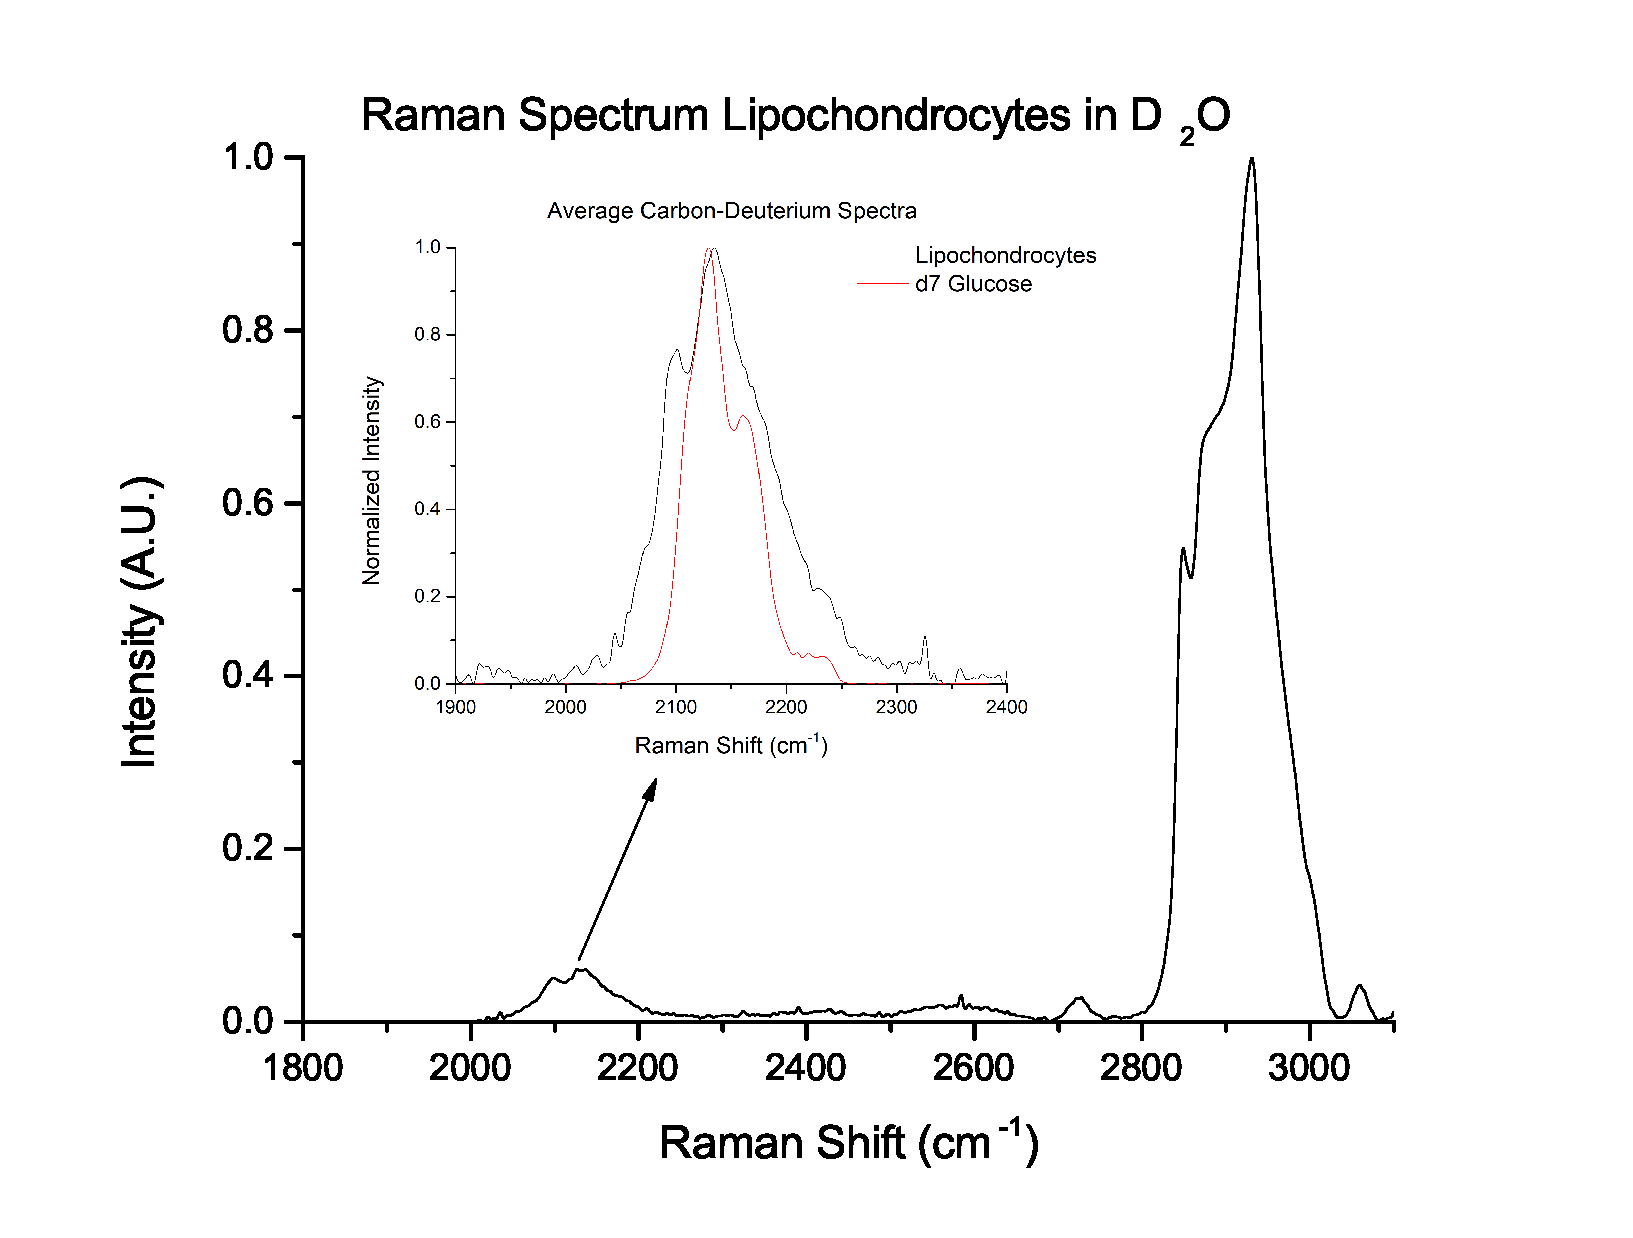
\includegraphics[width=1\linewidth]{Figures/Multigraph.eps}
    \caption{Caption}
    \label{fig:d7multiple}
\end{figure}

Previous work on the use of deuterium tagged molecules has been carried out by members of the Potma group as well as several other groups.~\cite{Hou2503,Alfonso-Garcia2015,Wei:2016aa}  The studies have indicated that deuterium is a useful tool as a contrast agent to mark specific compounds within cells and tissues. My work with the Potma lab was to extend this technique to the study of metabolism, with the lipochondrocyte as the cell model. Specifically, my research question was to examine whether or not the fate of deuterated carbon from a precursor molecule could be tracked in lipochondrocytes with SRS. The first indication that this would be a possibility is borne out in the Raman spectrum of deuterated glucose which is shown in the insert of \ref{fig:d7multiple}. In the first set of experiments excised tissue was cultured in media supplemented with d6-glucose for 48 hours.  The tissue was then fixed with $4\%$ paraformaldehyde and then rinsed.  The tissues were mounted between a standard microscope cover slide and a number 1 coverglass.  Raman spectra were taken from various points of multiple cells on a Renishaw InVia Raman Microscope at the UCI Laser Spectroscopy Facility. In the spectrum taken , we see an intense band centered around $\sim2900cm^{-1}$ from the averaged spectrum taken from the lipochondrocytes. This is attributed to the CH$_2$ stretching modes present in lipids and protein in the cells.  Another peak is present centered around $\sim2140cm^{-1}$  This peak corresponds to the C-D mode present in the cells.  This provides validation that SRS imaging of carbon-deuterium uptake is indeed possible.  The Raman spectrum of the CD modes obtained from the cells shows a marked change from the Raman spectrum of pure d6-glucose. This implies that d6-glucose has been chemically modified. The resulting spectrum shows features characteristic of deuterated lipid, thus suggesting that the majority of precursor molecules are likely converted to lipid-like compounds. 

\begin{figure}[h]
    \centering
    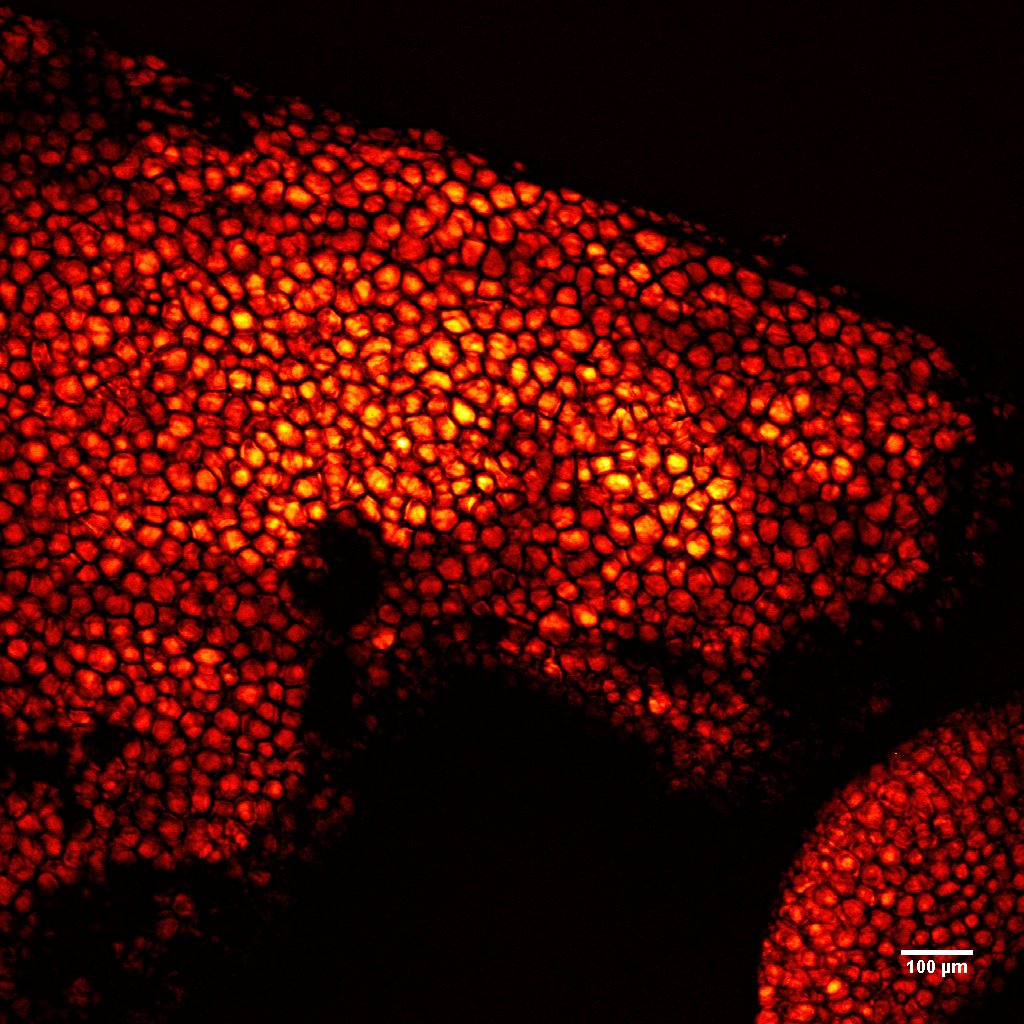
\includegraphics[width=0.5\linewidth]{Figures/2-methyl.jpg}
    \caption{Excised tissue imaged at the CH band.  Image shows primarily lipochondrocyte cells.}  
    \label{fig:Lipo-Methyl}
\end{figure}

After the initial spontaneous Raman study, SRS imaging was performed.  Initially, the system was tuned to the CH band around $\sim2900cm{^-1}$.  These images confirmed the presence of lipids in both control samples incubated with regular glucose and in those tissues cultured in the deuterated glucose media.  Figure \ref{fig:Lipo-Methyl} shows one such image from the deuterated sample set. The phase of the lock in demodulation is set prior to image acquisition to match the SRS signal of long chain fatty acids by first imaging a test sample of oil and adjusting lock-in settings to maximize the signal-to-noise ratio. The field of view of this image shows nearly all cells in this field of view are lipochondrocytes, and the contrast available at this band allows for discrimination of the cells from their surroundings. Figure \ref{fig:4chlipo} shows an image acquired at higher magnification. In this image it is possible to clearly see individual cells, and in some it is possible to see a dark region that is identified nucleus of the cell.  These images were compared with other tissues stained with Bodipy to identify concentrations of neutral lipids, and the same morphology is seen in both sets of samples.

\begin{figure}
    \centering
    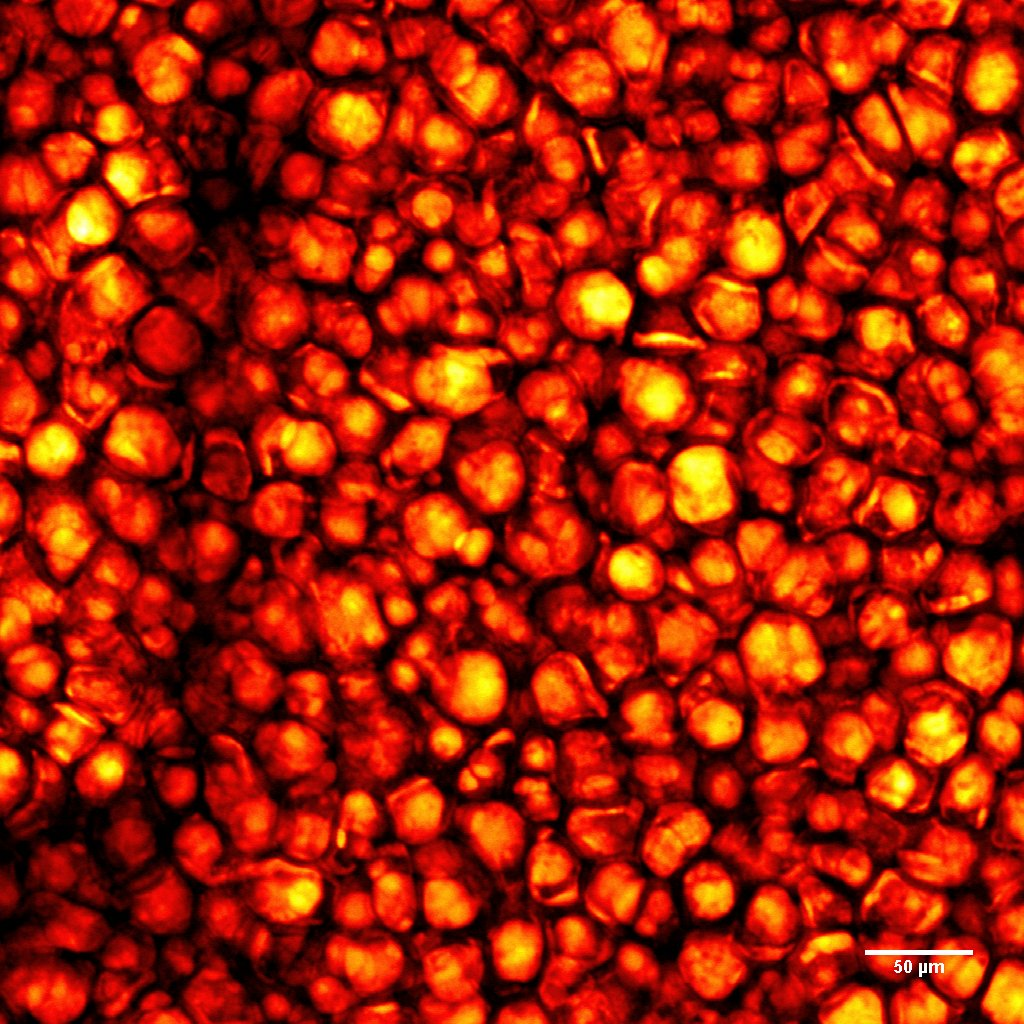
\includegraphics[width=0.5\linewidth]{Figures/4-methyl.jpg}
    \caption{Magnified view of lipochondrocytes imaged at the CH band.}
    \label{fig:4chlipo}
\end{figure}

After confirming morphology using the CH region, the SRS was tuned to probe the carbon-deuterium stretch around $\sim2140cm{^-1}$.  For signal optimization, a test sample of deuterated dimethyl sulfoxide was used, and demodulation of the lock in was phase locked to this signal.  Figure \ref{fig:compare} shows the results of one set of images.  Images were successfully acquired in the carbon deuterium band.  Overlay of the images show that the signal of the CD band is co-localized with the signal from the large lipid droplets. Further tests were performed in order to confirm that the signal is indeed from carbon-deuterium oscillators.  The large circular area in the center of the field of view is a collagen filled area.  In these images, it is devoid of cells, however in many instances these contain adipocytes.  Background images were acquired by tuning the OPO off-resonance from any known peak. These images were subtracted from the on-resonance images in order to improve the signal to noise ratio.  

\begin{figure}
    \centering
    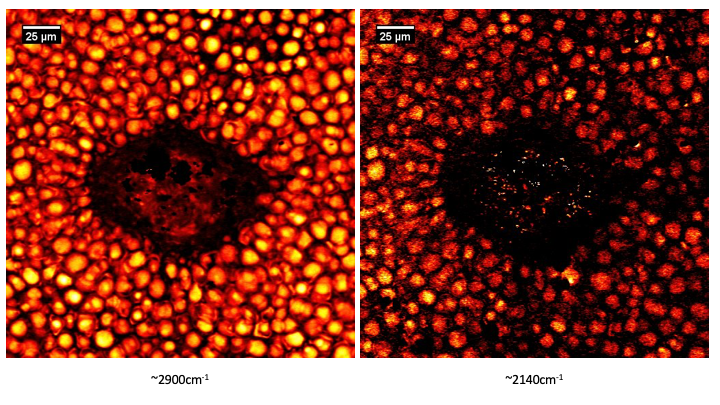
\includegraphics[width=\linewidth]{Figures/comparison.png}
    \caption{Lipochondrocytes imaged at both the CH, $\sim2900cm^{-1}$ and CD, $\sim2140cm^{-1}$ regions.  Images show colocalization of the lipid signal and the carbon deuterium signal}
    \label{fig:compare}
\end{figure}

These results lend evidence to the idea that lipid accumulation in lipochondrocytes occurs primarily through de novo lipogenesis as no significant amount of lipds are present in the growth media.  Images acquired at earlier time points in the incubation show decreased CD signal and decreased size of individual lipochondrocyte cells.  In addition to the control and CD groups presented here, our collaborators also performed experiments in which de novo lipogenesis was inhibited through application of C75 which inhibits synthesis of fatty acids. However, if lipid accumulation occurred through the ingestion of environmentally present lipids significant growth and signal would be expected to be present. Figure \ref{fig:pubfig} shows part of a figure intended for publication.  In it the average area of the ears of mice is calculated after application of a control of DMSO and several lipid inhibitors.  This evidence provided by the SRS experiments above lend credibility to the hypothesis that lipid accumulation in this cell type is through lipogenesis.

\begin{figure}
    \centering
    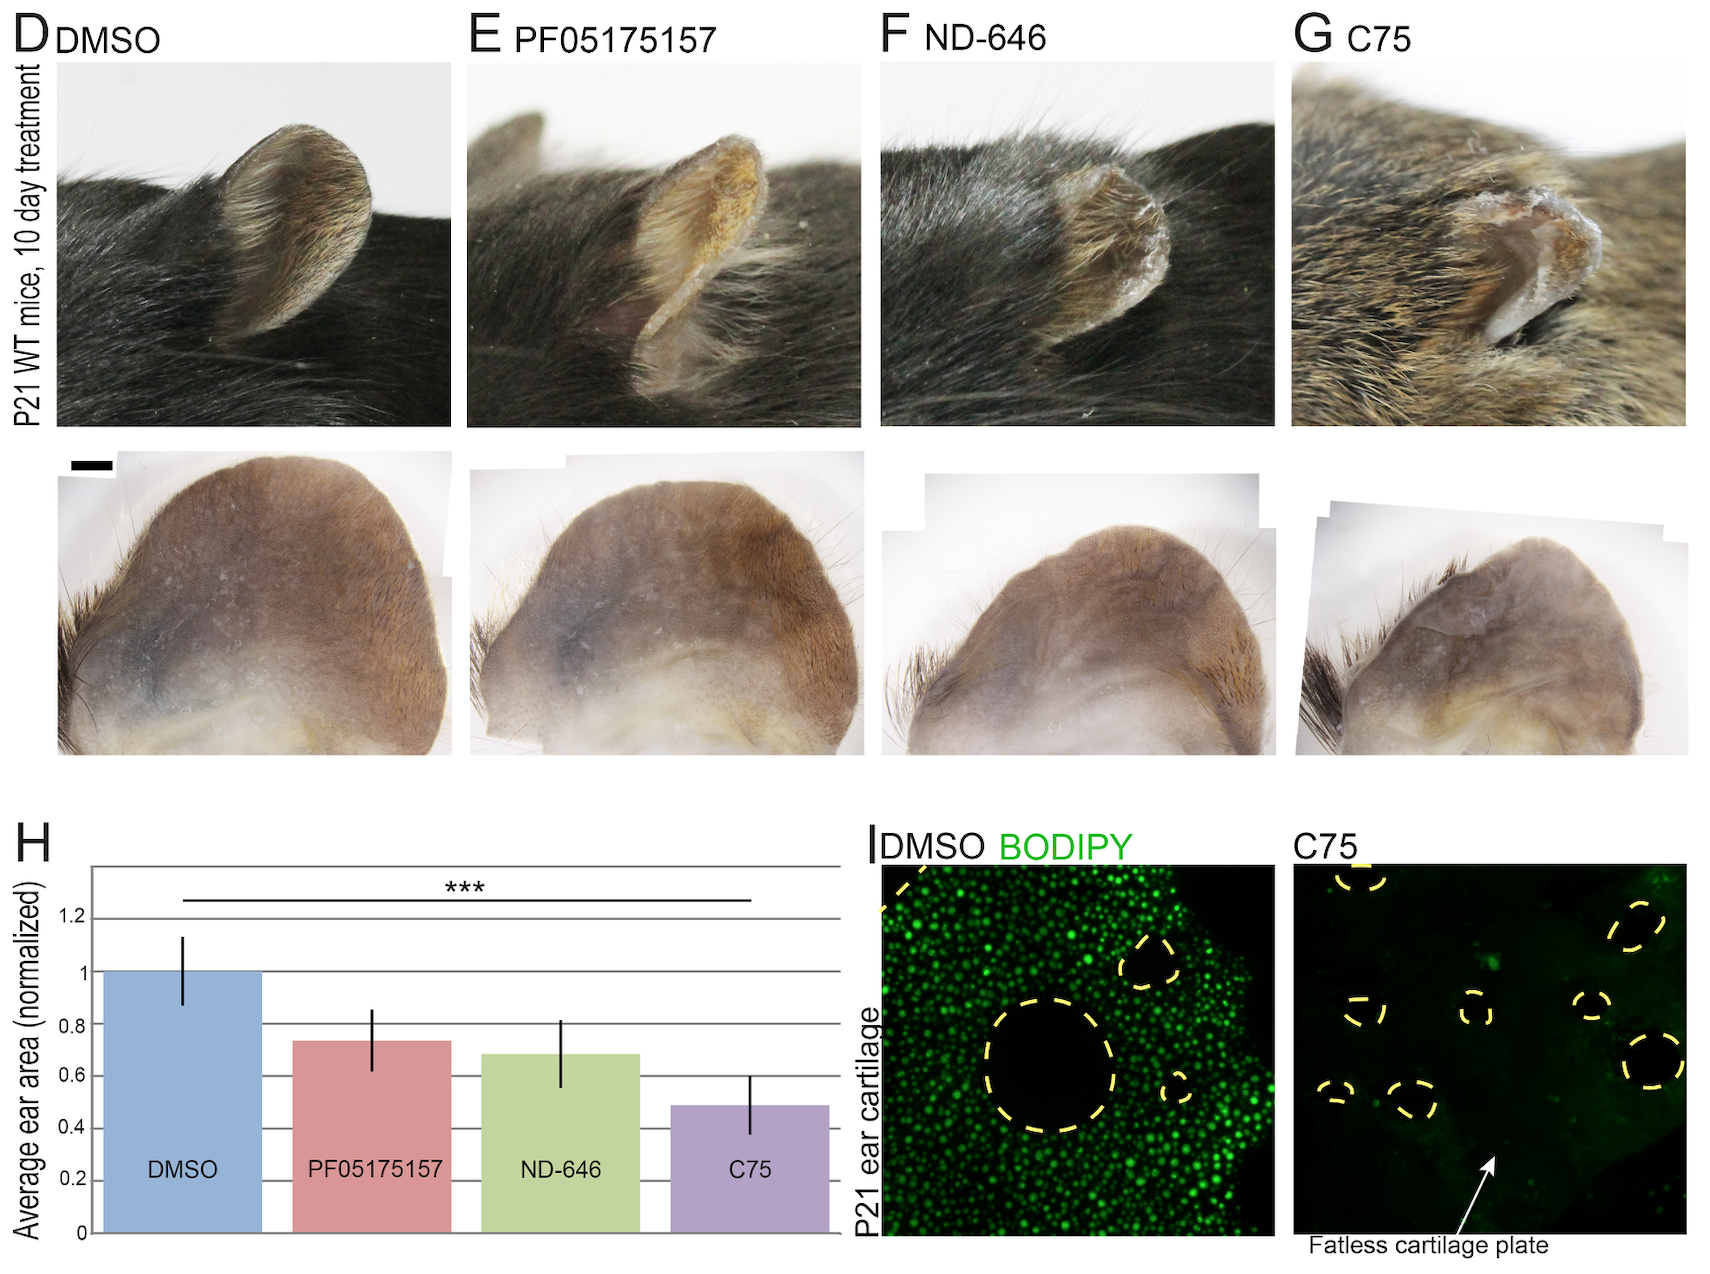
\includegraphics[width=\textwidth]{Figures/paperfig.png}
    \caption{Application of lipogenesis inhibitors to the ears of mice.  Application of C75 inhibits the production of fatty acids leading to deformed ears.}
    \label{fig:pubfig}
\end{figure}

\section{Aim 1: Elucidate diffusion dynamics of common cryoprotectants}
   The use of cryoprotectants to store cell cultures long term is well known, and has applications to fundamental and developmental biology, clinical medicine, stem cell treatments, and work on fertilization.\cite{EGLI2003352,SCHELLANDER1994909,JACOB198614}  Common chemicals used as such include glycerol and dilute concentrations of dimethyl sulfoxide.\cite{Pegg:2002aa}  While it has been established that these chemicals minimize ice crystal formation in the intracellular space, the mechanism by which this is accomplished is debated within the literature.\cite{nucleation1993} Glycerol and DMSO have both been shown to interact with the fusion of liposomes upon thawing, and the choice of cryopreservant can serious effect the viability of cells.~\cite{ANCHORDOGUY1987324, SCHELLANDER1994909} Figure \ref{fig:crystal} shows research on ice crystal formation in preserved cartilage cells images c and d show extensive damage after thawing from the formation of these crystals.~\cite{PEGG2010S36}
   
   Most of the SRS literature presents cases of research in which cells are fixed, or if live, the imaging is done on very specific cases.  In this project, I am proposing to use deuterated DMSO to perform flow based experiments on a variety of cell types.  To consider this project a success, I have identified three goals.  The first is to determine the diffusion coefficient of DMSO through the intracellular space. The results This parameter has been the subject of simulation.\cite{LEEKUMJORN20061751}  The second is to examine localized concentrations of DMSO within cells, and co-localize those concentrations with the distribution of organelles.  The final goal is to examine cells during standard thawing procedures to watch the outward diffusion of DMSO through the plasma membrane.  I expect that these experiments will provide new insights on the biophysical properties of small molecule cryopreservants. 
   
   \begin{figure}[h]
       \centering
       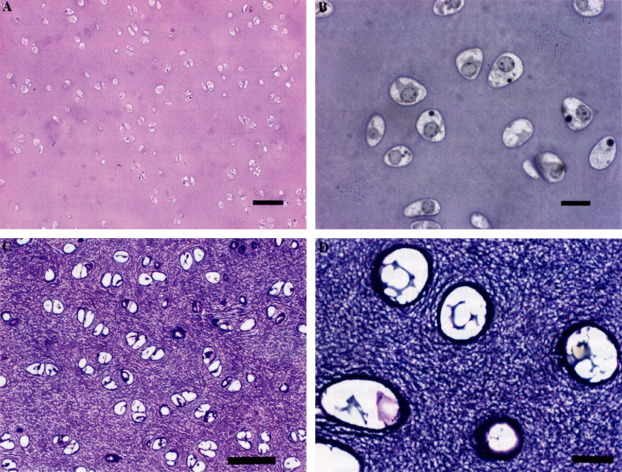
\includegraphics[width=.6\linewidth]{Figures/crystals.jpg}
       \caption{The appearance of control cartilage, sectioned and stained with toluidine blue, is shown in Panels A and B. Panels C and D show cartilage that was cooled to $ -80  \degree C$, freeze-substituted at that temperature, and also stained with toluidine blue. Note the large ice crystal cavities located in chondrons. ($bar = 50$ $\mu m$ in A and C, $bar = 10$ $\mu m$ in B and D) Modified from \cite{PEGG2010S36}.}
       \label{fig:crystal}
   \end{figure}
   
   Coherent Raman techniques have a history in the literature of being used for flow based experiments studying diffusion.  In 2001, CARS microscopy was used to study intracellular water diffusion.~\cite{Potma:2001aa}  Figure \ref{fig:flow} is from the 2001 work and provides an illustration of how the diffusion constant can be obtained through the use of coherent Raman techniques.  More recently in 2017 CARS was used to elucidate the barrier nature of the arterial wall, and was selected for commentary which was authored by myself and E. O. Potma. ~\cite{Lucotte4805, Prince201704101}  In both of these cases, deuterium oxide, heavy water, was used to provide the contrast necessary to follow the flow of water through the cells and tissue.  
   
   \begin{figure}[h]
       \centering
       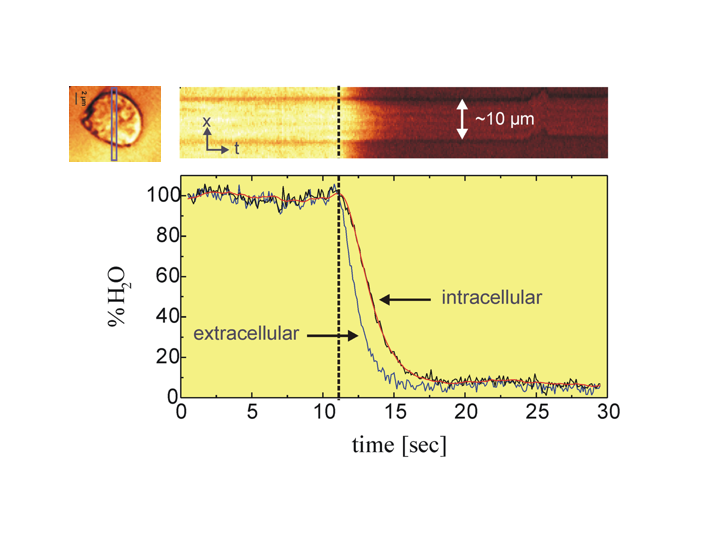
\includegraphics[width=\textwidth]{Figures/flow.png}
       \caption{Time based imaging of the flush of heavy water in the intracellular and extracelluar space. The time trace in the graph establish the flow of water prior to flush with deuterium oxide and post flush.  This allows for the diffusion time constant to be extracted.}
       \label{fig:flow}
   \end{figure}
   
   Early attempts at conducting this research have proven to be challenging.  As mentioned in the theory section, high-resolution SRS images without spurious background signals require the use of high numerical aperture objectives and condensers.  By definition, these optics have very small working distances.  For the purpose of flow experiments this limits the size of the fluidic systems that can be used. Imaging at steady state after introduction with deuterated DMSO reveals negative contrast in some areas of cultured MCF-7 cells.  This is shown in Figure \ref{fig:MCF7}  The low quality of this image shows that more work in engineering a suitable flow system is needed.
   
   
 \begin{figure}[h]
     \centering
     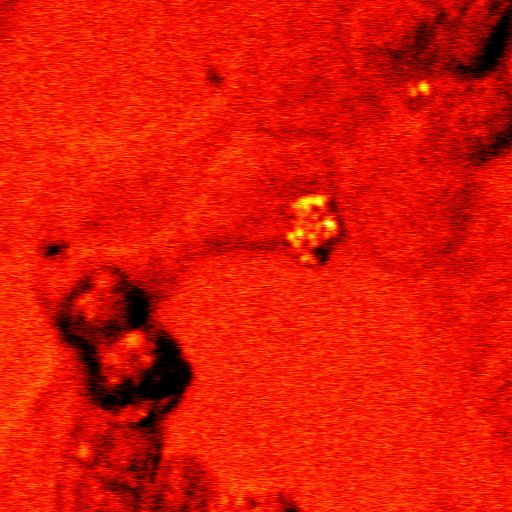
\includegraphics[width=.5\textwidth]{Figures/3DMSO.jpg}
     \caption{Imaging at the Carbon-Deuterium band reveals inhomogeneous distribution of DMSO through the intracellular space of several MCF-7 cells.}
     \label{fig:MCF7}
 \end{figure}

Current work on this project is focusing on the redesign of our flow cell system.  After several attempts at manufacturing a microfluidic system, a modification of a commercially available system from Bioptechs Corporation is being designed and manufactured. A schematic of the flow system is available in Figure \ref{fig:flowcell}.  The modifications to this system include widening the aperture on the condenser side to accommodate the space requirements of the high-NA condenser.  The system is being made thinner to accommodate the necessarily short working distances of the SRS system optics. Finally, a mounting plate is being designed and machined to accommodate the flow cell into the stage of the SRS microscope.   

\begin{figure}
    \centering
    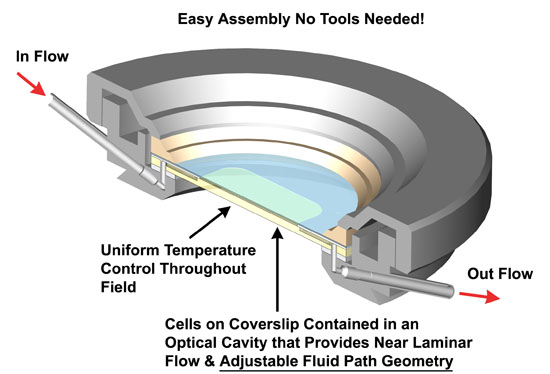
\includegraphics[width=.5\linewidth]{Figures/flowcell.jpg}
    \caption{Schematic of the Bioptechs flowcell system.}
    \label{fig:flowcell}
\end{figure}

Once the modifications to the flow cell design are accomplished, a process that should be completed by the end of this year, I intend to commence initial experiments with controlled flow.  The inclusion of shaped gaskets in the system allow for controlled nearly laminar flow over the cells.  Perfusion will be accomplished with the use of a syringe pump capable of pushing very low flow rate.  This will allow for repeatable imaging.  From a series of these experiments I expect to be able to collect data on the diffusion of deuterated DMSO across the plasma membrane thus accomplishing the first goal of this project.  

Extensive literature exists on the effects of DMSO on model membranes.\cite{ANCHORDOGUY1992117, GORDELIY19982343} Simple models based on Fink's law are commonplace in literature, and can be used as a starting point before expanding.\cite{LEEKUMJORN20061751} The literature has noted that it is quite common for the diffusion coefficient to be overestimated in small molecules.\cite{Evans:2018aa}  Common values for the diffusivity of DMSO in water range between 0.8 and 1.2 $x 10^-5 \frac{cm^2}{s}$\cite{IECR1992, doi:10.1002/cphc.201500670}  This rate is expected to be hindered based on the results described for intracellular water.

In order to accomplish the second goal of the project, only slight modifications to the SRS system should be necessary.  I intend to use cell cultures with various organelles tagged with fluorescent probes to study the accumulation of deuterated DMSO in and around various organelles. Simultaneous images between the SRS system and the fluorescent detection system will allow for this goal to be met. Interestingly enough in Figure \ref{fig:MCF7} high intensity spots can be seen in several of the MCF-7 cells.  Investigating these high concentration areas will determine what areas of the cell should be investigated in more detail.

Finally, the third goal of this project is to examine the reverse flow of DMSO out of preserved cells. This will be accomplished through the use of the heating element included with the flow cell. By monitoring the the thawing process it should be possible to understand if damage occurs to the cells prior to that point or during.  Additionally, experiments may be performed looking at the usual CH channel for lipids to monitor disruption in lipid droplet distribution during this process. 

It is anticipated that this project will commence in earnest in January 2019.  As stated above, the modifications to the flow system are already underway.  Once experiments begin, this project should take approximately 4 months to complete.  The largest factor with regards to time is maintaining proper cell cultures in order to have repeatable experiments.  Preliminary data should be available by the end of January and the project timeline will be examined and adjusted at that point.

\section{Aim 2: Demonstrate a method for metabolic sorting based on SRS imaging}

This project seeks to demonstrate a method for sorting inhomogenous cultures of cells based on metabolic signatures.  The idea for this project was encouraged through a serendipitous observation during the lipochondrocyte imaging project.  As shown in Figure \ref{fig:twocell} two different cell types are clearly visible.  The set of bright cells in the center of the dark region are immature adipocytes.  Despite the lipochondrocytes large concentration of lipids, the adipocytes are shown to have an even higher uptake of deuterated glucose and conversion to lipid.  This manifests in the much higher signal intensity shown in this image. The higher concentration of deuterated lipid signifies a higher metabolic rate of glucose consumption for the adipocyte cell relative to the lipochondrocyte cell. 

\begin{figure}[h]
    \centering
    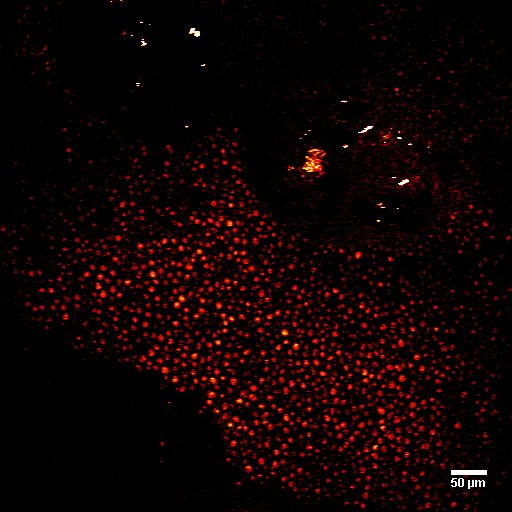
\includegraphics[width=0.7\textwidth]{Figures/twocell.jpg}
    \caption{Lipochondrocytes surrounding a small adipocyte.  Both cell types have been cultured in d6-glucose supplemented media.  However, the adiopocyte shows increased signal activity in the deuterium band.}
    \label{fig:twocell}
\end{figure}

In addition to the serendipitous result described above, recent work from the Min group at Columbia University has shown that by culturing cells in heavy water based media a fairly large number of deuterium based peaks show up in the normally silent region of the Raman spectrum.  These peaks can be measured rapidly and the intensity of them can be compared on a per cell basis. These ratios will then be used to devise an algorithm for classifying based on the metabolic rates represented by the Raman peaks.  Included in Figure \ref{fig:ming} are the results from the Min group showing the possibility of using several different deuterium modified functional groups for SRS imaging.~\cite{Shi:2018aa}

\begin{figure}[h]
    \centering
    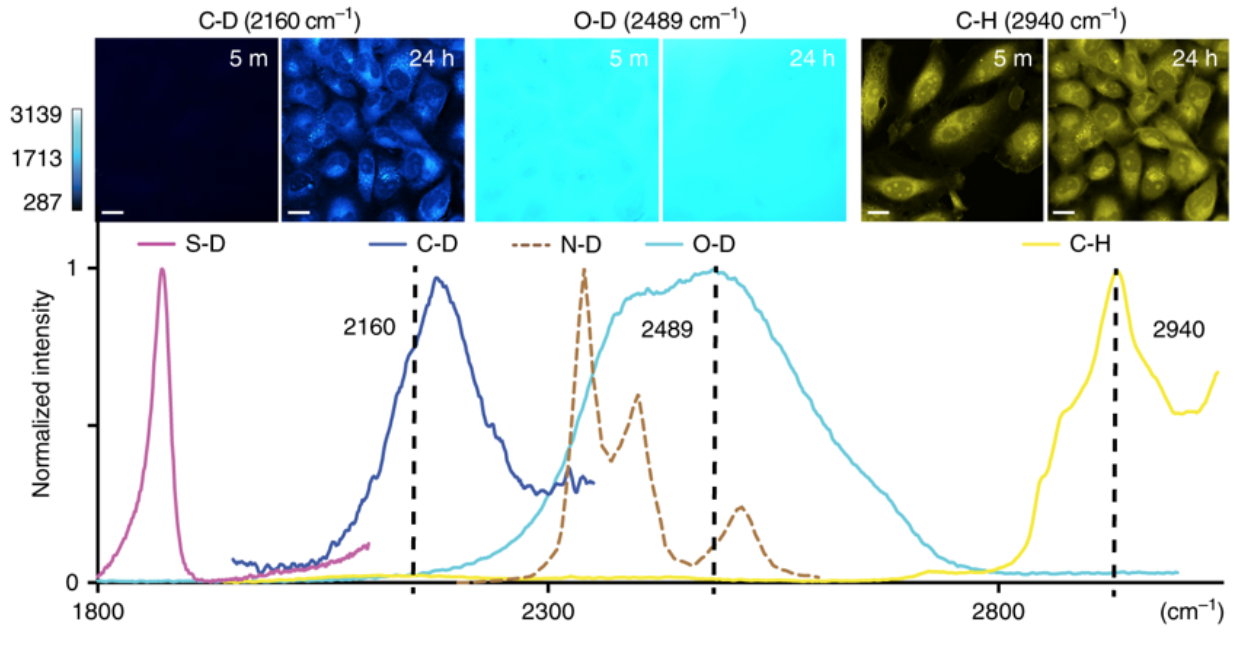
\includegraphics[width=\linewidth]{Figures/mingraph.png}
    \caption{Caption}
    \label{fig:ming}
\end{figure}

The first goal for this project is to measure the CD peak in a cancer cell line known to experience the Warburg effect, and compare this to a non cancerous line.  All cells will be grown with heavy water supplementation. Additionally, as long as the heavy water is kept at a low percentage of the overall media, the cells are not expected to experience significant isotope effects.  For the first series of experiments, the breast cancer line MDA-MB231 has been chosen.  This line shows increased metabolism as well as easily identifiable lipid droplets.  We will compare the results to cells derived from primary mammary epithelium, which represent healthy cells with a low glycolytic rate.  We expect that the overall amount of carbon-deuterium bonds is significantly different between the two cell types, which thus represents a marker for the metabolic activity of the cultures. The cell culture will be done in collaboration with the group of Prof. Robert Spitale

The second phase of this project will consist of examining mixed cultures of cells.  Cells with an increased metabolism phenotype will be cultured mixed with cells of a less active phenotype.  Using the data collected in the first phase, cells will be examined for the CD peak as well as any others that are found to be relevant.  A classification algorithm will be developed to increase the throughput of the system.  Validation at this step will consist of transfecting the high metabolism phenotype to express a fluorescent marker that can be imaged during the same session as SRS.  This process will be iterative until a high success rate is found.

The final phase of this project will consist of work with several collaborators to develop a microfluidic based sorting system.  In such a system, cells would be flowed through the focus of the microscope system. Based on the spectroscopic data collected previously, the algorithm will decide if the cell is high metabolism or low and the cell will be sorted into an appropriate bin.  Through fluorescent tagging of one of the two cell types this sorting system can also be validated in an iterative process.  

\section{Aim 3: Characterize Third-Order Sum-Frequency Generation as applied to biological systems}

In the past year, our group has published several papers on the development and demonstration of a new multi-modal microscope.\cite{Hanninen:18}  This system is capable of imaging using a new modality, third-order sum-frequency generation (TSFG) in addition to the already demonstrated modalities of SFG and CARS.  The Jablonski diagrams for these three modalities are shown in Figure \ref{fig:my_tsfg}.  In TSFG, molecules are driven at IR-active resonances but are probed through a hyper Raman interaction, effectively up-converting the signal from the IR to the visible range of the spectrum.  This is potentially revolutionary development as it allows IR-based imaging using collection and detection optics that are widely available for use in the visible range. In addition, the two-photon up-converting step confines the probing spot in three dimensions, producing a lateral resolution better than $0.5 \mu m$, many times below the IR-diffraction limit.  As this technique is only recently demonstrated, there remains a large about of work left to further characterize it.  

\begin{figure}
    \centering
    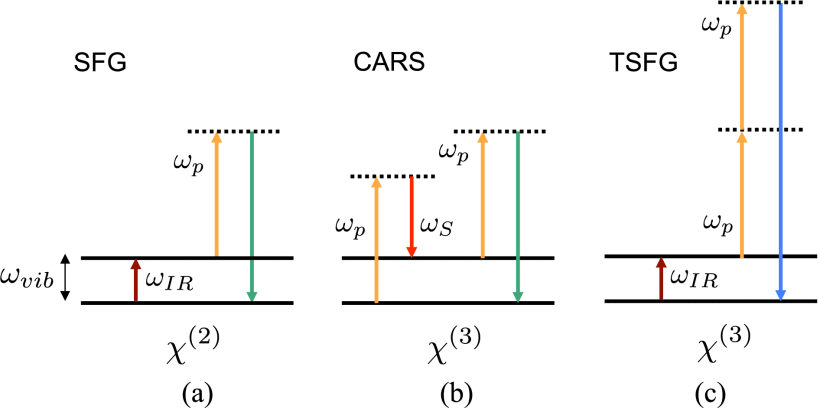
\includegraphics[width=\linewidth]{Figures/tsfg.png}
    \caption{Three different nonlinear optical interactions with vibrational sensitivity. (a) SFG, a second order process sensitive to modes with both Raman and IR activity; (b) CARS, a third order process sensitive to Raman active modes; (c) TSFG, a third order process sensitive to IR-active modes.}
    \label{fig:my_tsfg}
\end{figure}

Like the CRS techniques described above, TSFG depends on the  $\chi^(3)$ nonlinear susceptibility of the molecules under investigation.  Previous work on TSFG has shown that the response of commonly investigated substances like water and lipid have very different responses than would be expected from work done in CARS.  The non-resonant component of the signal is stronger in TSFG but varies from material to material. In order to characterize this, a series of spectral investigations will be carried out on common compounds that are expected to be probed by the microscope. Materials that are expected to be commonly encountered in TSFG experiments are representative solvents (water, ethanol, dimethyl sulfoxide, cyclohexane), biochemical structures (triglyceride, cholesterol, phospholipid, bovine serum albumin, collagen, cellulose, dextrose, DNA), polymer materials (polystyrene, polymethyl-methacrylate, melamine, polyvinyl alcohol), and inorganic materials (borosilicate glass, quartz, titanium oxide). The OPO that supports this system allows for spectral resolution at $\sim10cm{^1}$, and the spectra will be collected over a range of 2080 to 4000 $cm^{-1}$.  These spectra will be correlated with spectra collected from UV/Vis and FTIR.  The UV spectra correlation will provide information on the effect of proximity to electronic resonances on the TSFG response.  The FTIR spectra will serve to inform the resonant response of the material much as the spontaneous Raman spectra does in SRS or CARS investigations.

The second phase of investigations with this system will be its application to biological systems.  In particular, this system will be applied to work from our longstanding collaboration with Prof. James Jester (Ophthalmology, UCI), which focuses on the distribution and composition of lipids in the meibomian gland.  Meibum has previously been investigated with SRS, and those studies revealed new information about the distribution of protein and lipid in meibum with applications towards understanding dry eye disease.  Hyperspecral imaging through TSFG will provide protein/lipid distribution maps.  These will be compared and correlated with the maps originally derived from SRS investigations.  This will reveal additional information about the composition of the lipids in the meibomian gland and their role in the tear film layer of the eye.

The timeline for this project will commence during the second half of 2019.  At that point, collection of data on the various compounds will commence.  This part of the project along with optimization of the TSFG system itself will last for the remainder of the year.  Collection of UV/Vis data and FTIR will be conducted at the UCI Laser Spectroscopy Facility and will be conducted by a pair of highly trained undergraduate students currently working in the lab.  This will free graduate researcher time to focus on the TSFG system itself. Work on the meibum system will commence in early 2020 and last for an expected six months.
